\section{調査}
\subsection{動画・画像の活用割合}
図\ref{content_trend}は,動画及び画像の活用割合の推移である.
2016年までは,画像の活用は0.01\%未満であり,動画に関しては0件であった.
2017年以降,活用件数は急激に増加し,2021年には,動画~0.72\%,画像~5.93\%であった.
2017年に急激に増加した要因に関しては調査中である.

\begin{figure}[t]
  \begin{center}
      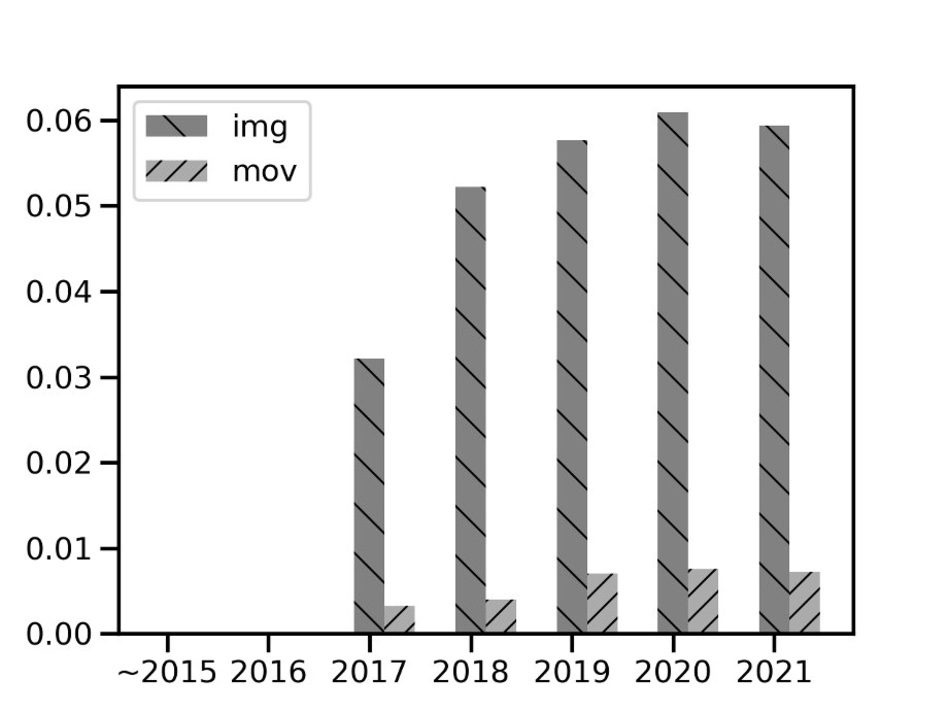
\includegraphics[scale=0.45]{./image/data_content_trends.pdf}
      \caption{動画・画像の活用割合推移 \label{content_trend}}
  \end{center}
\end{figure}

\subsection{データの分析}

\begin{figure*}[t]
  \begin{center}
      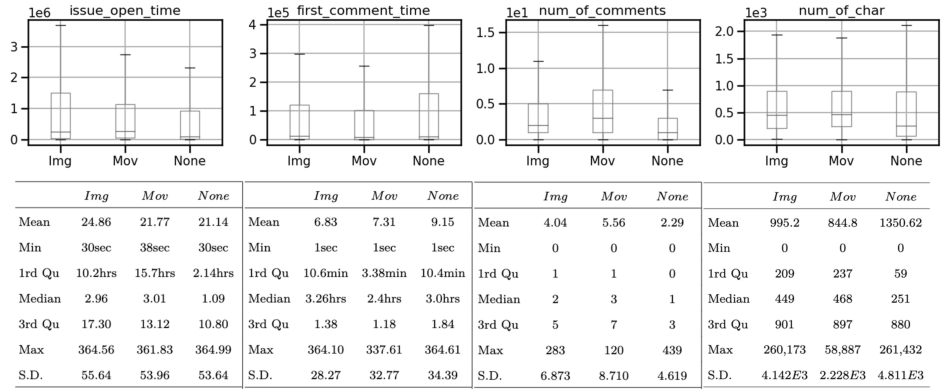
\includegraphics[scale=1.1]{./image/dataset_plot.pdf}
      \caption{Issue群ごとの調査項目の分布及び代表値 \label{dataset_plot}}
  \end{center}
\end{figure*}

図\ref{dataset_plot}は,データの特性値を箱ひげ図及び表で表現したものである.
ただし,図\ref{dataset_plot}の箱図の最大値は,$3rd~Qu + 1.5 * IQR$以下の最大値である.
($IQR$:四分位範囲)% この様な処理は,データの中央値付近を見やすくする為にしばしば用いられる.

動画及び画像を含むIssueは,そうでないIssueに比べて,
$Issue\_open\_time$が平均で,2.9\%\textasciitilde17.6\%増加し,
$Num\_of\_comments$が平均で76.4\%\textasciitilde143\%増加した.
一方で,$First\_comment\_time$が平均で20.1\%\textasciitilde25.4\%減少し,
$Num\_of\_char$が平均で26.3\%\textasciitilde 37.5\%減少した.

\noindent{\bf{正規性について.}}
%図\ref{dataset_plot}では,$Issue\_open\_time$,$First\_comment\_time$及び$Num\_of\_char$の平均値が,
%四分位範囲内に収まっていないことから正規分布から逸脱している.
%$Num\_of\_comments$に関しては,正規分布しているような印象を受ける.
%実際,$Img$の平均値 = 4.04,標準偏差$S.D.$ = 6.873であり,これから$\pm~3S.D.$の上限値は24.66と算出できる.
%これから,最大値283は外れ値であるとも考えられる.しかし,
Kolmogorov-Smirnov検定の結果,すべての項目に対して,正規性は有意水準0.05で棄却された.
\\
\noindent{\bf{等分散性について.}}
$Leneve$検定の結果を表\ref{levene_result}に示す.
帰無仮説は「すべてのIssue群間を通して等分散」であり,有意水準は0.20とする.

\begin{table}[h]
  \begin{center}
  \caption{等分散性検定の結果}
  \begin{tabular}{l|r c} 
    \hline
     & 有意確率 & 平均分散比 \\ 
    \hline \hline
    $Issue\_open\_time$ & 0.378 & 1.050 \\
    $First\_comment\_time$ & 0.296 & 1.301 \\
    $Num\_of\_comments$ & *~0.001 & 2.459 \\
    $Num\_of\_char$ & *~0.073 & 3.156 \\
    \hline
  \end{tabular}\\
  \small
    *~ : 有意水準0.20で有意\\
  \label{levene_result}
  \end{center}
\end{table}

$Num\_of\_comments$及び$Num\_of\_char$は,等分散性が有意水準0.20で棄却される.
$Issue\_open\_time$及び$First\_comment\_time$は,有意確率が有意水準以上であることと,
平均分散比が~1~\textasciitilde ~1.5~程度であることから,等分散性を仮定する.


\subsection{統計的検定}
ここでの検定の目的は,各調査項目の群間の分布の差が統計的に有意であるかを確かめることである.
5.2節において,正規性及び等分散性を満足しない調査項目が含まれることを確かめた.
従って,検定には,正規性及び等分散性を仮定しないSteel-Dwass法を用いる.
Steel-Dwass法による検定結果を表\ref{Steel-Dwass_result}に示す.
有意水準は0.05とする.

\begin{table}[t]
  \begin{center}
  \caption{調査項目ごとの多重比較の結果}
  \begin{tabular}{l r|r}
    \hline
    調査項目 & 対 & 有意確率 \\
    \hline \hline
    $Issue\_open\_time$ & & \\
     & \bf{$Img$~vs~$None$} & **~0.002 \\
     & \bf{$Mov$~vs~$None$} & **~0.021 \\
     & \bf{$Img$~vs~$~Mov$} & 0.381 \\
    \hline
    $First\_comment\_time$ & & \\
     & \bf{$Img$~vs~$None$} & 0.764 \\
     & \bf{$Mov$~vs~$None$} & 0.351 \\
     & \bf{$Img$~vs~$~Mov$} & 0.404 \\
    \hline
    $Num\_of\_comments$ & & \\
     & \bf{$Img$~vs~$None$} & *~0.001 \\
     & \bf{$Mov$~vs~$None$} & *~0.001 \\
     & \bf{$Img$~vs~$~Mov$} & 0.211 \\
    \hline
    $Num\_of\_char$ & & \\
     & \bf{$Img$~vs~$None$} & *~0.001 \\
     & \bf{$Mov$~vs~$None$} & *~0.001 \\
     & \bf{$Img$~vs~$~Mov$} & 0.599 \\
    \hline
  \end{tabular}\\
  \small
    *~ : 両側検定で有意 ~~~ ** : 片側検定で有意\\
  \label{Steel-Dwass_result}
  \end{center}
\end{table}

$Img$及び$Mov$は,$None$に比べて,$Issue\_open\_time$が有意に大きく,
$Num\_of\_comments$及び$Num\_of\_char$については分布に何らかの有意な差があると解釈できる.
一方で,$First\_comment\_time$においては,有意差は認められなかった.
また,$Img$と$Mov$の比較では,すべての項目で有意差は認められなかった.
%有意差が認められなかった項目については,有意差の有無の判断を保留する.

\subsection{出現単語分析}
ここでの目的は,各Issue群のIssueにどのような単語が含まれているかを明らかにすることである.
各Issueの出現単語を\textbf{tf\_idf}値に変換し,Issue群ごとに結合した.
各Issue群の\textbf{tf\_idf}値上位10単語を表\ref{tf-idf_result}に示す.
"at"や"it","the"などの単語を除外する為,
名詞,動詞及び疑問詞のみを対象とした.

$Img$では"image"や"screen"など表示に関係する単語が多く,
$Mov$では"dropdown"や"button"など動きのある表示に関する単語が多い.
一方で,$None$では,リポジトリの管理に関する単語が多く,
プルリクエストやコミットに関する通知報告がなされていると推察される.
$Mov$では"when"が1番目に,$Img$でも3番目にランクインした.これは,不具合の再現に関する報告である可能性が高い.
実際に,目視調査で,不具合の再現動画が多いことを実験的に確かめた.
一方で,$None$では1番目に"dependabot"がランクインした.DependaBotは,最新のライブラリを推奨したり更新するボットであり,
設定により自動でIssueを生成することもある.
$Img$及び$Mov$と$None$の差は,ボットによる影響を受けている可能性がある.

\begin{table}[t]
  \begin{center}
  \caption{Issue群ごとの\textbf{tf\_idf}上位10単語}
  \begin{tabular}{r | c c c }
     & $Img$ & $Mov$ & $None$\\
    \hline \hline
    1 & image & when & dependabot\\
    2 & screenshot & dropdown & code\\
    3 & when & view & file\\
    4 & error & package & pullrequest\\
    5 & screen & issue & version\\
    6 & version & python & error\\
    7 & shot & height & use\\
    8 & file & react & lib\\
    9 & test & button & add\\
    10& code & text & commit\\
  \end{tabular}\\
  \label{tf-idf_result}
  \end{center}
\end{table}